\DiaryEntry{Heapsort}{2020-01-24}{Algorithms}

Heapsort's running time is $\Oc(n \log n)$ and it is also an in-place sorting algorithm.

Equally interesting is that heapsort intoduces a ``heap'' data structure, which is pretty useful and which can be used to implement an efficient priority queue.


\subsection {Heaps}

The (binary) heap data structure is an array object which represents a tree structure. An example is shown in the following Figure. Each array elements corresponds to a tree node. The tree is completely filled at all levels but the last (filled from left to right and stops ``somewhere''). Given the index $i$ of a node, its left and right siblings can be calculated according to

\begin{verbatim}
left(i) = 2*i
right(i) = 2*i+1
\end{verbatim}

whereas the index of the parent is given by

\begin{verbatim}
parent(i) = floor(i/2)
\end{verbatim}


\begin{figure}[hbt!]
\centering
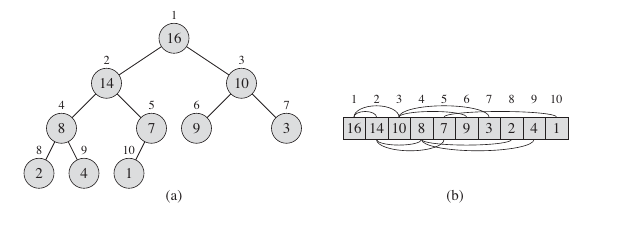
\includegraphics[scale=0.7]{images/heapsort_1.png}
\end{figure}

There are two kind of heaps: Max-heaps and min-heaps. In a max-heap, the nodes fulfill the following max-heap property,

\begin{verbatim}
A[parent(i)] >= A[i]
\end{verbatim}

I.e. the parent is larger or equal than its siblings. Therefore, the largest element is at the root. Analoguously, the min-heap fulfills the min-heap property,

\begin{verbatim}
A[parent(i)] <= A[i]
\end{verbatim}


The \emph{height of a node} is the number of edges on the longest simple downward path from the node to a leaf. The \emph{height of a heap} is the height of its root node. If the heap has $n$ elements, its height is $\log_2 n$.

In the following, we consider three algorithms,

\begin{itemize}
\item The max-heapify algorithm, which maintains the max-heap property for a subtree.
\item The build-max-heap algorithm, which produces a max-heap from an unordered input array.
\item The heapsort algoithm, which sorts an array in place.
\end{itemize}

The Julia implementations can be found \href{https://github.com/ClemensFMN/JuliaStuff/blob/master/algorithms/heapsort.jl}{here}).

\subsection{Max-Heapify Algorithm}

The max-heapfiy algorithm considers the node A[i] and its two siblings, A[left(i)] and A[right(i)]. It asusmes that the binary trees rooted at A[left(i)] and A[right(i)] fulfill the max-heap property. The algorithm searches the maximum of A[i], A[left(i)], and A[right(i)]; if the maximum is A[i] it is finished as the max-heap property has been already fulfilled. In the two other cases (one of the siblings is the maximum), it replaces the A[i] with the sibling. Then it applies the max-heapify algorithm to the subtree.

The running time is $\Oc(\log n)$; the exchange has constant complexity and max-heapify needs to run $\Oc(\log n)$ times (down to the bottom of the tree).

\paragraph{Example.} As an example, we consider the following binary tree

\begin{figure}[H]
\centering
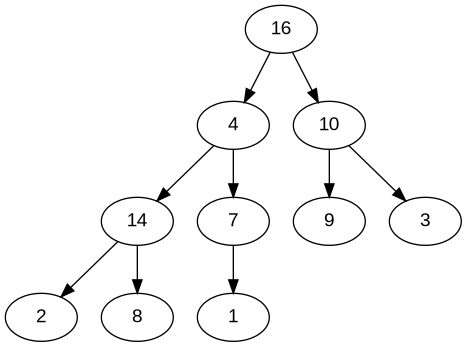
\includegraphics[scale=0.5]{images/heapsort_2.png}
\end{figure}

Note that only the $4$ is ``wrong''; in particular, the subtrees left and right below the $4$ satisfy the max-heap property. In a first step, the $4$ is `exchanged with the $14$, yielding the following tree.

\begin{figure}[H]
\centering
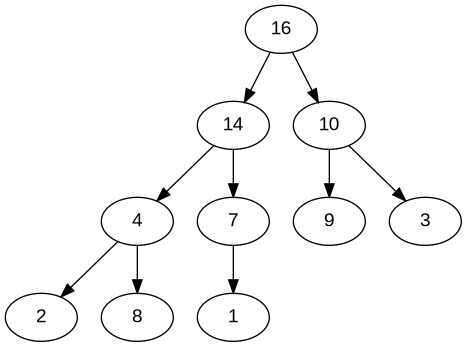
\includegraphics[scale=0.5]{images/heapsort_3.png}
\end{figure}

Now we continue the subtree which root was changed (that's the left one) and run max-heapify with the new root $4$. We exchange $4$ with $8$ and finally arrive at the following tree. 

\begin{figure}[H]
\centering
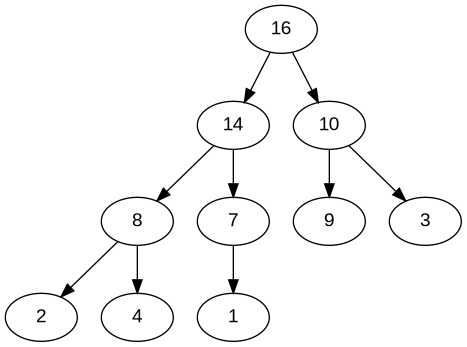
\includegraphics[scale=0.5]{images/heapsort_4.png}
\end{figure}

\qed


\subsection{Build-Max-Heap Algorithm}

We can use the max-heapify algorithm bottom up to convert an unordered array into a max-heap. We note that the elemnts in the second half of the earray $A[\lfloor n/2 \rfloor \ldots n]$ are the siblings. We therefore start the max-heapify algorithm at $A[\lfloor n/2 \rfloor]$ and work upwards to $A[1]$.

\paragraph{Example.} We consider a slightly different example of the following tree

\begin{figure}[H]
\centering
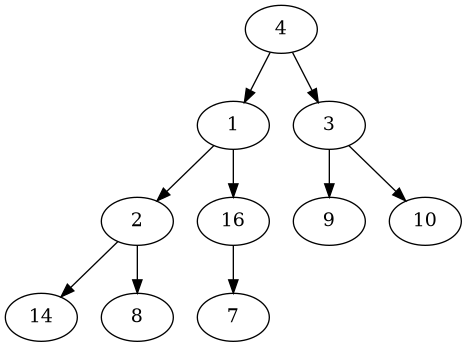
\includegraphics[scale=0.5]{images/heapsort_10.png}
\end{figure}

We first start withth meax-heapifying the tree at node $16$; since this subtree already has the max-heap property, nothing changes.

\begin{figure}[H]
\centering
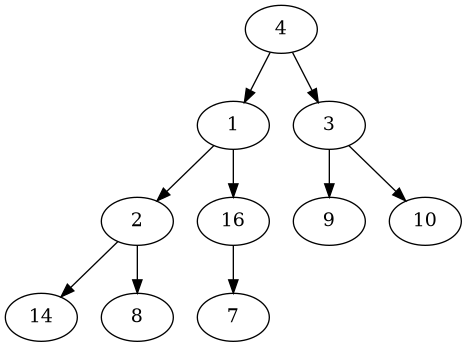
\includegraphics[scale=0.5]{images/heapsort_11.png}
\end{figure}

The subtree with root $2$ is max-heapified, yielding

\begin{figure}[H]
\centering
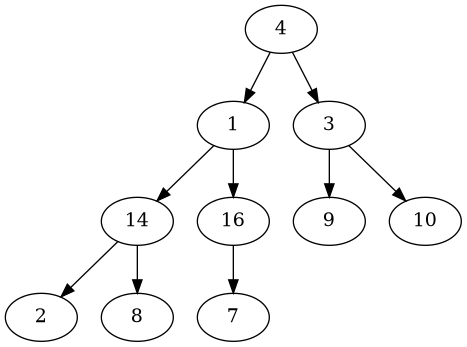
\includegraphics[scale=0.5]{images/heapsort_12.png}
\end{figure}

Now we go onle level up, and consider the subtree with root at $3$.

\begin{figure}[H]
\centering
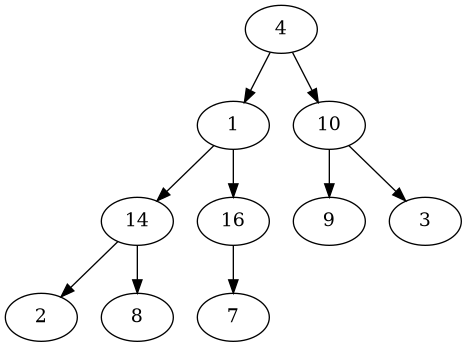
\includegraphics[scale=0.5]{images/heapsort_13.png}
\end{figure}

The subtree with root $1$ is processed next, yielding a big change in the left subtree.

\begin{figure}[H]
\centering
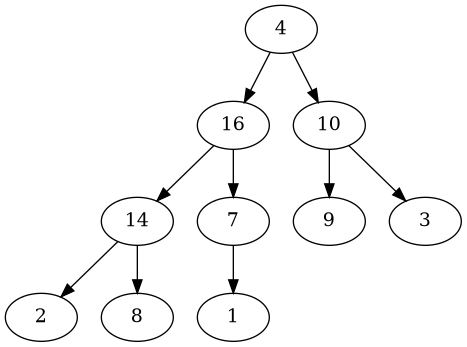
\includegraphics[scale=0.5]{images/heapsort_14.png}
\end{figure}

And finally, we consider the root of the tree, yielding

\begin{figure}[H]
\centering
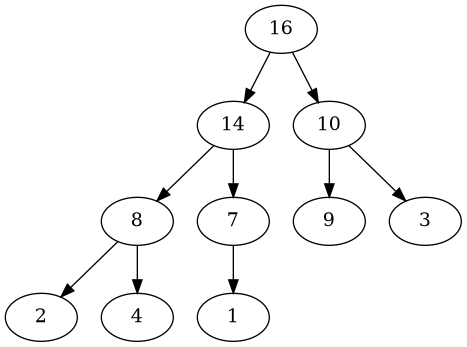
\includegraphics[scale=0.5]{images/heapsort_15.png}
\end{figure}

\qed

\subsection{Heapsort Algorithm}

The heapsort algorithm uses the fact that the root of the tree contains the maximum element. We start with applying the build-max-heap algorithm to the whole array, which yields the maximum elements at the root. In the next step, we exchange A[1] with A[n] and consider a tree of size $n-1$. The new tree root might violate the max-heap property, therefore we restore it via the max-heapify algorithm. Now A[1] holds the largest element of the tree (and the seocnd largest element of the array to be sorted), so we replace A[1] with A[n-2] and continue. until we have a tree of size $1$.

\paragraph{Example}

We consider the following tree after the first max-heapify procedure

\begin{figure}[H]
\centering
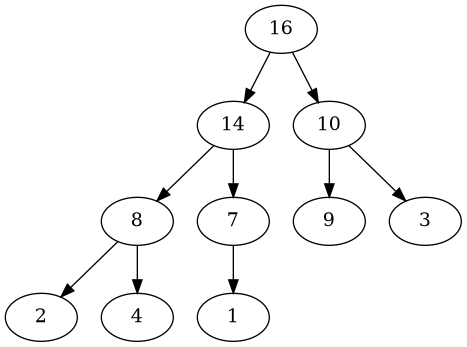
\includegraphics[scale=0.5]{images/heapsort_20.png}
\end{figure}

Now we remove the root $16$ and run max-heapify, yielding.

\begin{figure}[H]
\centering
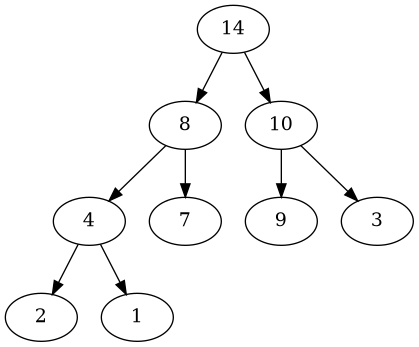
\includegraphics[scale=0.5]{images/heapsort_21.png}
\end{figure}

Removing $14$ yields the following tree

\begin{figure}[H]
\centering
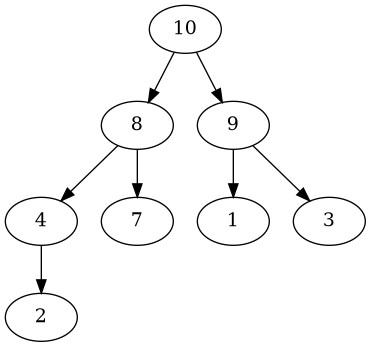
\includegraphics[scale=0.5]{images/heapsort_22.png}
\end{figure}

and so on and on. The sequence of removed tree roots is a sorted.



\qed


%%% Local Variables:
%%% mode: latex
%%% TeX-master: "journal"
%%% End:
